
This section will display what deliverables the testing will produce.

\subsection{Before Testing}
\begin{itemize}
    \item Test Plan - this document
    \item{Test Cases specification}
    \item{Test Design specification}
\end{itemize}
Test Cases and Test Design are put into the gitlab boards as seen in figure 1 and 2. An example of a test case specification for the tests that are possible from our current development in software can be seen in X. All test cases are derived from requirements and each requirement can have many test cases. The requirements are moved to different labels depending on its status.  




\subsection{During Testing}
\begin{itemize}
    \item Tests
\end{itemize}
The tests are added to the gitlab issue board via requirements issues as mentioned before. For the actual code part of the tests those can be found in the branch testingBranch in the gitlab associated with the project. 
\begin{itemize}
    
    \item{Test Data}
\end{itemize}
Is added in the gitlab issue board together with Test Results. If a test comes out as failed or not even ran, this will be added to issues in gitlab, where development will be tagged together with the log from the test.
\begin{itemize}

    \item{Test Traceability}
\end{itemize}
Test Traceability can be seen in the gitlab issue boards, where passed tests will be put to the closed issue area and will then be added as a regression test. Every test will be named according to the requirement they are testing, so if a test fails its easy to fix the coding faults.

\subsection{After Testing}
\begin{itemize}
    \item Test Result
\end{itemize}
Is added to the gitlab issue connected to the test case together with Test Data. Every test result will be marked as either passed or failed, together with a log if it does fail.

\begin{figure}

    \centering
    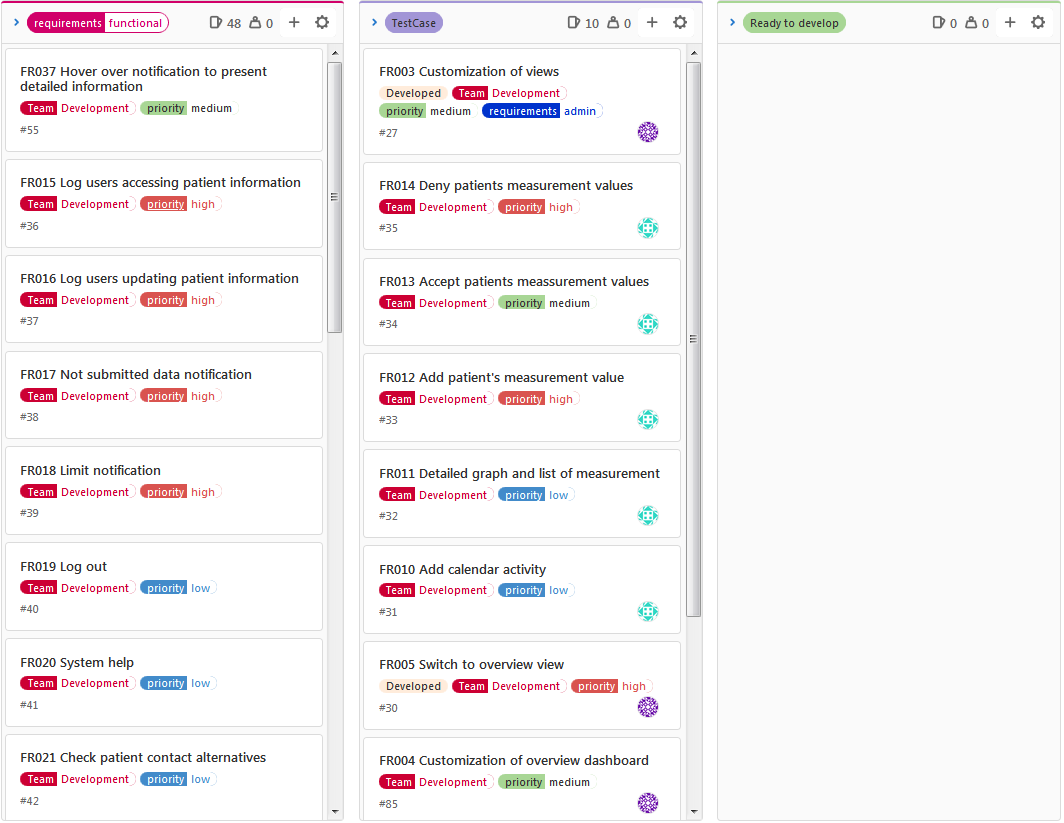
\includegraphics[scale=0.5]{Pictures/gitlab.PNG}
    \caption{Gitlab boards}
\end{figure}
\begin{figure}

    \centering
    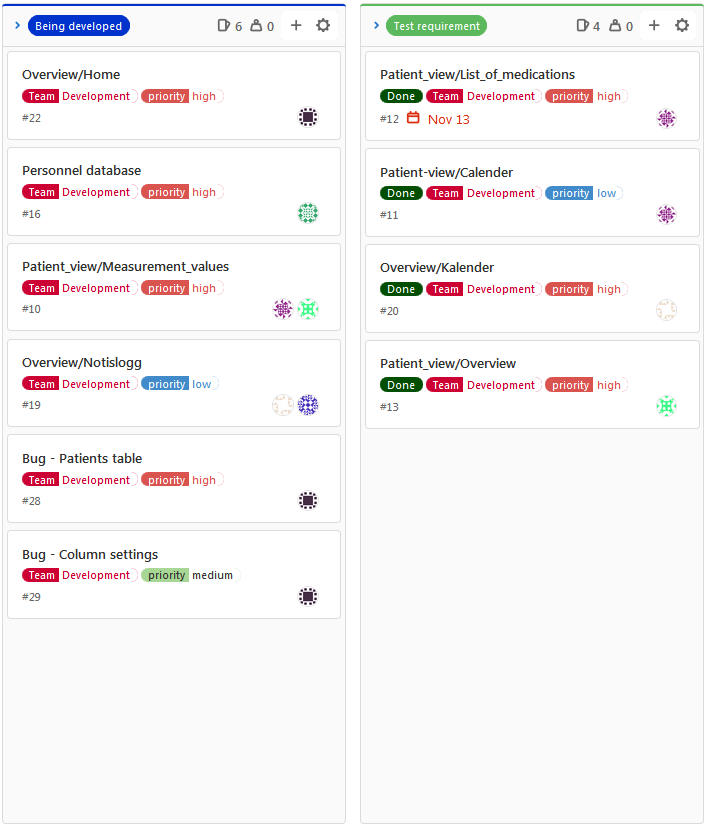
\includegraphics[scale=0.5]{Pictures/gitlab2.PNG}
    \caption{Gitlab boards}
\end{figure}
\begin{figure}

    \centering
    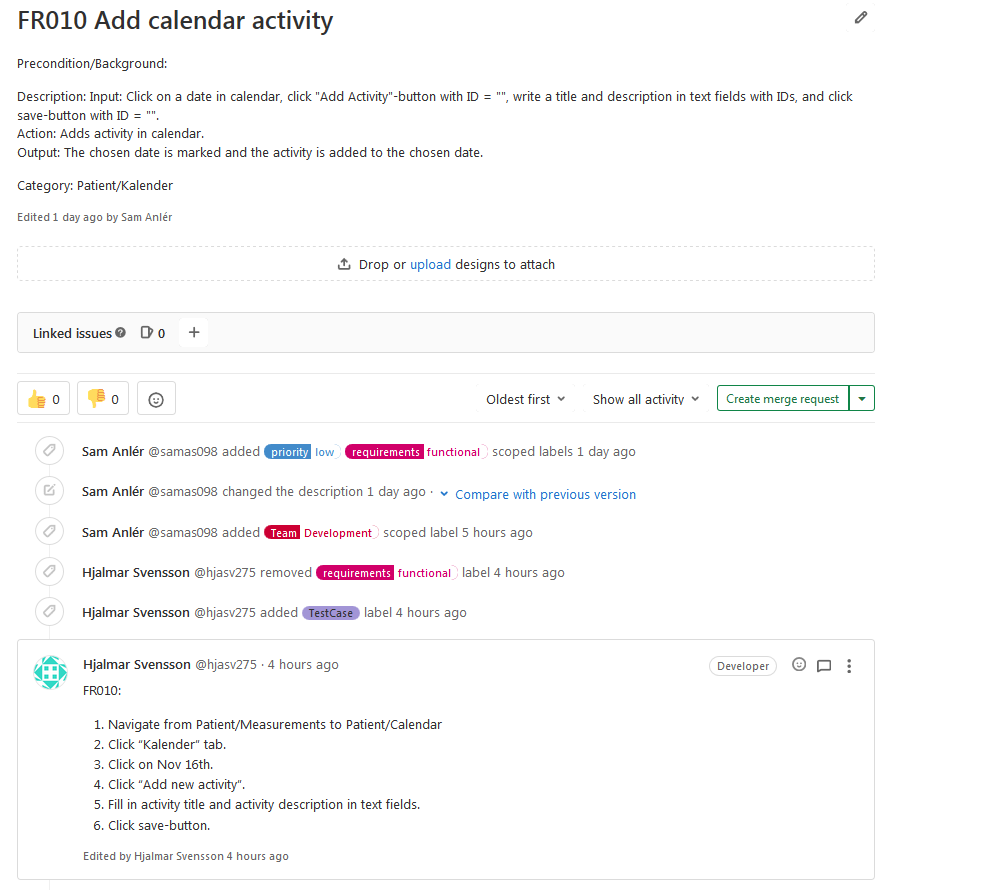
\includegraphics[scale=0.75]{Pictures/TestCase1.PNG}
    \caption{Test case for requirement}
\end{figure}
\subsection{Schedule}
\vfill
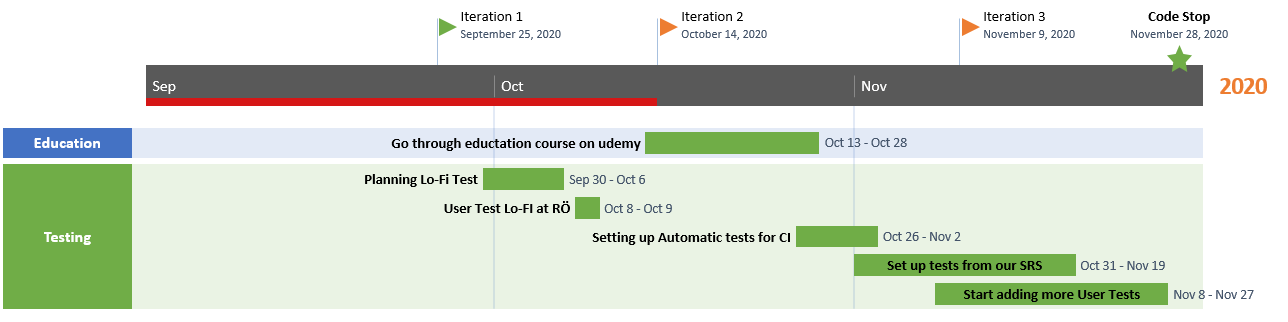
\includegraphics[width=\linewidth]{Pictures/TestSchedule.PNG}

    \vfill
\clearpage
